\section{Návrh metódy}
Navrhovaná metóda zohľadnuje vlastnosti ktoré nie je možné získať iba z videa, budeme ich nazívať dynamické príznaky videa.
Avšak metóda stále zohľadnuje v pozorovanom videu aj aspekty statického obrazu, tieto budeme nazívať statické príznaky videa.
Tieto príznaky sú vypočítavané seprátne a nakoniec ich metóda spája do jednej výslednej mapy pozornosti. Výsledkom je postupnosť máp pozornosti pre každý frame videa (podľa vstupnej konfigurácie), ktorý možno spojiť do videa pozornosti pre vstupné video.

\subsection{Dynamické príznaky videa}
Dynamické príznaky metóda najprv extrahuje pomocou štadardnej metódy Horn-Schunck, (referencia na 2 kapitolu alebo na článok?) ktorá vypočíta optický tok na 2 rozdielnych framoch videa čím vzniká sémantický príznak pohybu rôznych objektov po scéne spolu s smerovýmy vektormy pohybu daných vektorov.
Získané smerové vektory okamžite spočítavame aby sme získali celkový obraz optického toku pre danú dvojicu obrazov.
Obraz sa následne prahuje statickou konštantou kôli ostráneniu šumu. V našej implementácií sme použili prah v absolútnej hodnote (0.2) pre každý obrazový pixel vo výslednom optikom toku.
Pixeli s valídnou honotou sa rozdelia na regióny podľa spojitosti a podobnosti štandardným spôsobom.
Pripomenme, že v tomto obraze sa spočítali hodnoty posunu v oboch smeroch aritmeticky do jednej hodnotiacej konštanty (pre každý pixel obrazu), ktorá už nereprezentuje smer posunu daného obrazového pixelu, ale iba hodnotí celkový posun pixelu.
Takto získané regóny budeme vyhodnocovať a spájať podľa pôvodných výsledkov metódy Horn-Schunck.
Vďaka využitiu pôvodných vektorov z výsledku metódy Horn-Schunck, vieme rozlíšiť pohyb horizontálny aj vertikálny separátne.
Pre všetky dvojice regiónov v obraze zistujeme nasledovné charakteristiky:
\begin{enumerate}
  \item\textbf{Rozdiel smerových vektorov v horizontálnom smere}
  \item\textbf{Rozdiel smerových vektorov v vertikálnom smere}
  \item\textbf{Rozdiel vo vzdialenosti}
\end{enumerate}
\subsubsection{Rozdiel smerových vektorov v horizontálnom smere}
Charakteristika sa vypočítava zo smerových horizontálnych vektorov metódy Horn-Schunck.
Prekazdý región sa vypočíta maximálna hodnota z indexov daného regiónu.
Následne sa za hodnotu chrakteristiky sa považuje absolútna hodnota rozdielu týchto hodnôt.

\begin{figure}[H]
  \begin{equation}
    hodnota_A = max(hor_{vektory}(indexy_A))
  \end{equation}
  \begin{equation}
    hodnota_B = max(hor_{vektory}(indexy_B))
  \end{equation}
  \begin{equation}
    rozdiel_{horizontalny} = abs(hodnota_A-hodnota_B)
  \end{equation}
  \caption{vypočet hodnôt pre dvojicu regiónov}
  \vspace{10mm}
\end{figure}

\subsubsection{Rozdiel smerových vektorov v vertikálnom smere}
Charakteristika sa vypočítava zo smerových vertikálnych vektorov metódy Horn-Schunck.
Prekazdý región sa vypočíta maximálna hodnota z indexov daného regiónu.
Následne sa za hodnotu chrakteristiky sa považuje absolútna hodnota rozdielu týchto hodnôt.

\begin{figure}[H]
  \begin{equation}
    hodnota_A = max(ver_{vektory}(indexy_A))
  \end{equation}
  \begin{equation}
    hodnota_B = max(ver_{vektory}(indexy_B))
  \end{equation}
  \begin{equation}
    rozdiel_{vertikalny} = abs(hodnota_A-hodnota_B)
  \end{equation}
  \caption{vypočet hodnôt pre dvojicu regiónov}
  \vspace{10mm}
\end{figure}

\subsubsection{Rozdiel vo vzdialenosti}
Chrakteristika sa vypočítava ako minimálna hodnota vzdialenosti medzi dvojicou regiónov.
Hodnota je počítaná euklidovskou metódou.

\begin{figure}[H]
  \begin{algorithm}[H]
   \ForAll{rohA ako každý extrém regiónu A}{
     \ForAll{rohB ako každý extrém regiónu b}{
      vzdialenost = sqrt( (corner2(1,1)-rohB(1,1))^2 + (rohB(1,2)-rohA(1,2))^2 ) \\
     }
   }
   \caption{Výpočet minimálnej vzdialenosti euklidovskou metódou}
  \end{algorithm}
  \vspace{10mm}
\end{figure}

\subsubsection{Spájanie regiónov}
Po výpočte všetkých 3 charakteristík spojíme všetky dovjice regionov, pre ktoré su všetky chrakteristyky nižšie ako zadefinovaná konštanta.
Regióny spájame pomocou konvexného obalu zjednotenia bodov ležiacich v oboch regiónoch.
\begin{figure}[H]
  \centering
  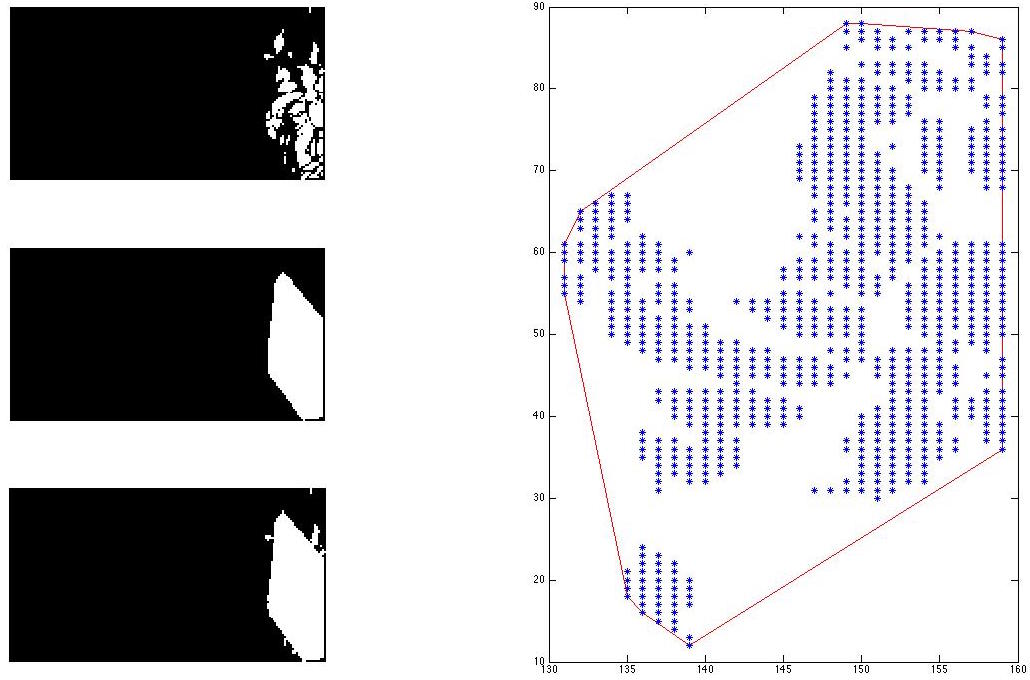
\includegraphics[width=15cm]{pics/spojenie-regionov.jpg}
  \caption{Vyzualizácia spojenia regiónov pomocou konvexného obalu}
  \vspace{10mm}
\end{figure}

\subsubsection{Starnutie objektov na scéne}
Do vypočitavnia dynamických príznakov započítavame predpoklad, že aj pohybujúce sa objekty postupne strácajú pozornosť používateľov.
A to v prípade kedy sa síce daný objekt na scéne pohybuje, ale na identickom mieste.
do metóty zabudujeme mechanizmus kde pixelom s dlhodobo vysokým hodnotením pozornosti, zmenšíme toto hodnotenie pomocou  vynásobenia koeficientom hodnoty \numrange{0}{1}.

\subsection{Statické príznaky videa}
Pri videách kde sa pohybuje celá scéna (kamera je v pohybe) nedávajú dynamické príznaky dobré výsledky kdeže logicky označia celú scénu alebo jej vädšinovú časť scény za výrazne salientnú.
Preto je vhodné dynamické príznaky vhodne kombinovať s klasickýmy modelmy pozornosti ktoré síce zanedbajú postupnosť obrazov, ale nezlyhajú ako dynamické príznaky.
Pre extrakciu statických obrázkov sme zvolili metódu založnú na spektralnych reziduach\cite{spectral-rezidual}.
Vďaka svojmu príncípu potlačovania štatisticky opakujúcich sa predmetov na scéne, sa dá predpokladaď vhodné doplnenie statických objektov ktoré možu zaujať pozornosť na videu ak zlyhávajú dynamické príznaky.

\subsection{Výsledné spojenie príznakov}
Spájanie dynamických a statických príznakov bude prebiehat pomocou sčítania oboch máp, pričom vždy s použijú u určitom pomere.
Výpočet pomeru bude určovať pomer výskytu salientných pixelov v mape dynamických príznakov.

\begin{figure}[H]
  \begin{equation}
    pomer = (sum(dynamickéPríznaky} > 0))/početElementov(dynamickéPríznaky)
  \end{equation}
  \caption{vypočet pomeru salientných pixelov v obraze}
  \vspace{10mm}
\end{figure}

Ak je vysoký výskyt salientých pixelov, potrebujeme utlmit zobrazovanie tejto časti príznakov a prioritizovať zobrazovanie statických priznakov preto zmišavacia funkcia vyzerá nasledovne:

\begin{figure}[H]
  \begin{equation}
    mapa_{pozornosti} = (dynamickéPríznaky * (1-pomer)) + (statickéPríznaky * pomer)
  \end{equation}
  \caption{zmiešavacia funkcia statických a dynamických príznakov}
  \vspace{10mm}
\end{figure}

\subsection{Pipeline metódy}
  TODO nakoniec wokflow diagram.

\section{Implementácia riešenia}
\section{Validácia výsledkov}
\section{Možnosti pre zlepšenie}
\section{Diskusia}
